\chapter{chapter A: Lorem ipsum dolor sit amet, consectetuer adipiscing elit.}
\lipsum[1]

\section{Introduction}
\lipsum[2-3]

\section{Background and Thread}
\lipsum[4-5]

\subsection{Backgroud}
\lipsum[6-7]

\subsection{Thread}
\lipsum[6-7]

%-------------------------------------------------------------------------------
\section{Footnotes, Verbatim, and Citations}
%-------------------------------------------------------------------------------

Footnotes should be places after punctuation characters, without any spaces between said characters and footnotes, like so.\footnote{Remember that USENIX format stopped using endnotes and is now using regular footnotes.} And some embedded literal code may look as follows.\par

\begin{verbatim}
int main(int argc, char *argv[]) 
{
    return 0;
}
\end{verbatim}

Now we're going to cite somebody. Watch for the cite tag. Here it comes. Arpachi-Dusseau and Arpachi-Dusseau co-authored an excellent OS book, which is also really funny~\cite{arpachiDusseau18:osbook}, and Waldspurger got into the SIGOPS hall-of-fame due to his seminal paper about resource management in the ESX hypervisor~\cite{waldspurger02}.\par

The tilde character (\~{}) in the tex source means a non-breaking space. This way, your reference will always be attached to the word that preceded it, instead of going to the next line.\par

And the `cite' package sorts your citations by their numerical order of the corresponding references at the end of the paper, ridding you from the need to notice that, e.g, ``Waldspurger'' appears after ``Arpachi-Dusseau'' when sorting references alphabetically~\cite{waldspurger02,arpachiDusseau18:osbook}.\par 

It'd be nice and thoughtful of you to include a suitable link in each and every bibtex entry that you use in your submission, to allow reviewers (and other readers) to easily get to the cited work, as is done in all entries found in the References section of this document.\par

Now we're going take a look at Section~\ref{sec:figs}, but not before observing that refs to sections and citations and such are colored and clickable in the PDF because of the packages we've included.\par

%-------------------------------------------------------------------------------
\section{Floating Figures and Lists}
\label{sec:figs}
%-------------------------------------------------------------------------------

\begin{figure}
\begin{center}
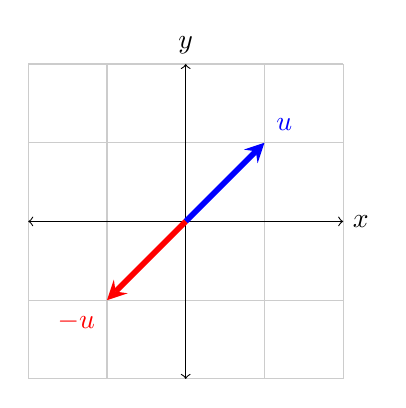
\begin{tikzpicture}
  \draw[thin,gray!40] (-2,-2) grid (2,2);
  \draw[<->] (-2,0)--(2,0) node[right]{$x$};
  \draw[<->] (0,-2)--(0,2) node[above]{$y$};
  \draw[line width=2pt,blue,-stealth](0,0)--(1,1)
    node[anchor=south west]{$\boldsymbol{u}$};
  \draw[line width=2pt,red,-stealth](0,0)--(-1,-1)
    node[anchor=north east]{$\boldsymbol{-u}$};
\end{tikzpicture}
\end{center}
\caption{\label{fig:vectors} Text size inside figure should be as big as caption's text. Text size inside figure should be as big as caption's text. Text size inside figure should be as big as caption's text. Text size inside figure should be as big as caption's text. Text size inside figure should be as big as caption's text. }
\end{figure}

Here's a typical reference to a floating figure: Figure~\ref{fig:vectors}. Floats should usually be placed where latex wants then. Figure\ref{fig:vectors} is centered, and has a caption that instructs you to make sure that the size of the text within the figures that you use is as big as (or bigger than) the size of the text in the caption of the figures. Please do. Really.\par

In our case, we've explicitly drawn the figure inlined in latex, to allow this tex file to cleanly compile. But usually, your figures will reside in some file.pdf, and you'd include them in your document with, say, \textbackslash{}includegraphics.\par

Lists are sometimes quite handy. If you want to itemize things, feel free:\par

\begin{description}
  
\item[fread] a function that reads from a \texttt{stream} into the array \texttt{ptr} at most \texttt{nobj} objects of size \texttt{size}, returning returns the number of objects read.

\item[Fred] a person's name, e.g., there once was a dude named Fred who separated usenix.sty from this file to allow for easy inclusion.
\end{description}

\noindent
The noindent at the start of this paragraph in its tex version makes it clear that it's a continuation of the preceding paragraph, as opposed to a new paragraph in its own right.\par


\subsection{LaTeX-ing Your TeX File}
%-----------------------------------

People often use \texttt{pdflatex} these days for creating pdf-s from tex files via the shell. And \texttt{bibtex}, of course. Works for us.\par

%-------------------------------------------------------------------------------
\section*{Acknowledgments}
%-------------------------------------------------------------------------------

The USENIX latex style is old and very tired, which is why there's no \textbackslash{}acks command for you to use when acknowledging. Sorry.\par

%-------------------------------------------------------------------------------
\section*{Availability}
%-------------------------------------------------------------------------------

USENIX program committees give extra points to submissions that are backed by artifacts that are publicly available. If you made your code or data available, it's worth mentioning this fact in a dedicated section.\par

\chapter{chapter B: long chapter title name\\ with line break}
\lipsum[8-12]

\section{System Overview}
\lipsum[9-13]

\section{Design and Implementation}
\lipsum[11-15]

\begin{appendices}
\chapter{chapter C}
\lipsum[13]

\section{app A}
\lipsum[14-15]

\section{Codes}
\begin{lstlisting}[language=Python]
import numpy as np
    
def incmatrix(genl1,genl2):
    m = len(genl1)
    n = len(genl2)
    M = None #to become the incidence matrix
    VT = np.zeros((n*m,1), int)  #dummy variable
    
    #compute the bitwise xor matrix
    M1 = bitxormatrix(genl1)
    M2 = np.triu(bitxormatrix(genl2),1) 

    for i in range(m-1):
        for j in range(i+1, m):
            [r,c] = np.where(M2 == M1[i,j])
            for k in range(len(r)):
                VT[(i)*n + r[k]] = 1;
                VT[(i)*n + c[k]] = 1;
                VT[(j)*n + r[k]] = 1;
                VT[(j)*n + c[k]] = 1;
                
                if M is None:
                    M = np.copy(VT)
                else:
                    M = np.concatenate((M, VT), 1)
                
                VT = np.zeros((n*m,1), int)
    
    return M
\end{lstlisting}

\rinput{../color-palette.tex}
% %-------------------------------------------------------------------------------
\section{Color Palettes}
%-------------------------------------------------------------------------------

% Color Palette (HTML)
%------------------------------------------------------------------------------
\newcommand\cp[1]{%
\textcolor[HTML]{#1}{\rule{10pt}{10pt}}
~\hspace{5pt}
~\parbox[c][10pt][c]{60pt}{#1}
}
\newcommand\csep{%
\hspace{1pt}
}

%-------------------------------------------------------------------------------
\subsection{Single Color}

\cp{3b0084}\csep
\cp{7474e0}\csep
\cp{191035}
\par

%-------------------------------------------------------------------------------
\subsection{Multi-Color}

% documents
\begin{enumerate}
\item
\cp{005e9a}\csep
\cp{ff8400}\csep
\cp{fed9d9}
\item
\cp{334854}\csep
\cp{e04463}\csep
\cp{efecea}\csep
\cp{f99055}\csep
\cp{e56cd6}
\item
\cp{ed1010}\csep
\cp{ff5151}\csep
\cp{ffa0a0}\csep
\cp{be0d71}\csep
\cp{0a8d8e}
\item
\cp{d01114}\csep
\cp{f9b700}\csep
\cp{f0e1b8}
\item
\cp{427dcd}\csep
\cp{c0b9af}\csep
\cp{fcdac6}
\item
\cp{005e9a}\csep
\cp{ff8400}\csep
\cp{fed9d9}
\item
\cp{e8643c}\csep
\cp{d4c045}\csep
\cp{98ccdd}
\item
\cp{427dcd}\csep
\cp{c0b9af}\csep
\cp{fcdac6}
\item
\cp{ab7e49}\csep
\cp{0c3f5a}\csep
\cp{f0cfa8}\csep
\cp{ab5f49}\csep
\cp{347954}
\item
\cp{f5502f}\csep
\cp{0382fe}\csep
\cp{fbcb00}
\item
\cp{1c37ee}\csep
\cp{ff4400}\csep
\cp{d8d0cd}
\item
\cp{567990}\csep
\cp{4277bb}\csep
\cp{bec4cf}
\item
\cp{cf211e}\csep
\cp{464646}\csep
\cp{dddddd}\csep
\cp{f99055}\csep
\cp{e56cd6}
\item
\cp{f9b70e}\csep
\cp{244d67}\csep
\cp{f1d796}\csep
\cp{f98c0e}\csep
\cp{666ab7}
\item
\cp{ab7e49}\csep
\cp{0c3f5a}\csep
\cp{f0cfa8}\csep
\cp{ab5f49}\csep
\cp{347954}
\item
\cp{ff3366}\csep
\cp{0c3f5a}\csep
\cp{45e1d3}\csep
\cp{20a4f3}\csep
\cp{979797}
\item
\cp{334854}\csep
\cp{e04463}\csep
\cp{efecea}\csep
\cp{328080}\csep
\cp{9fc84e}
\item
\cp{d01114}\csep
\cp{f9b700}\csep
\cp{f0e1b8}
\item
\cp{737495}\csep
\cp{f17d81}\csep
\cp{e7efde}\csep
\cp{d6bd9d}\csep
\cp{677b89}
\item
\cp{334854}\csep
\cp{e04463}\csep
\cp{efecea}\csep
\cp{20a4f3}\csep
\cp{979797}
\item
\cp{cf211e}\csep
\cp{464646}\csep
\cp{dddddd}
\item
\cp{f9b70e}\csep
\cp{244d67}\csep
\cp{f1d796}\csep
\cp{f98c0e}\csep
\cp{666ab7}
\item
\cp{5749d9}\csep
\cp{ae6bdf}\csep
\cp{2eecf8}\csep
\cp{fff33b}\csep
\cp{e968bc}
\item
\cp{86bcd8}\csep
\cp{c1bd97}\csep
\cp{a8c1ce}\csep
\cp{7d637e}\csep
\cp{99ad88}
\item
\cp{334854}\csep
\cp{e04463}\csep
\cp{efecea}
\item
\cp{aced15}\csep
\cp{a1918e}\csep
\cp{b4adea}\csep
\cp{bebbbb}\csep
\cp{ef798a}
\item
\cp{616161}\csep
\cp{1dc2e5}\csep
\cp{aeebdb}\csep
\cp{ffab1a}\csep
\cp{ff571a}
\item
\cp{4e828b}\csep
\cp{71aaa7}\csep
\cp{b6d8d5}
\item
\cp{5749d9}\csep
\cp{ae6bdf}\csep
\cp{2eecf8}
\item
\cp{cf211e}\csep
\cp{464646}\csep
\cp{dddddd}\csep
\cp{328080}\csep
\cp{9fc84e}
\item
\cp{ff3366}\csep
\cp{0c3f5a}\csep
\cp{45e1d3}\csep
\cp{20a4f3}\csep
\cp{979797}
\item
\cp{00adb5}\csep
\cp{0c3f5a}\csep
\cp{f8b500}\csep
\cp{ff0700}\csep
\cp{979797}
\item
\cp{567990}\csep
\cp{4277bb}\csep
\cp{bec4cf}\csep
\cp{94ae89}\csep
\cp{896978}
\item
\cp{f9b70e}\csep
\cp{244d67}\csep
\cp{f1d796}\csep
\cp{ff0700}\csep
\cp{979797}
\item
\cp{567990}\csep
\cp{4277bb}\csep
\cp{bec4cf}\csep
\cp{94ae89}\csep
\cp{896978}
\item
\cp{00adb5}\csep
\cp{0c3f5a}\csep
\cp{f8b500}\csep
\cp{ff0700}\csep
\cp{979797}
\item
\cp{00adb5}\csep
\cp{0c3f5a}\csep
\cp{f8b500}\csep
\cp{ff0700}\csep
\cp{979797}
\item
\cp{ebb200}\csep
\cp{a5a5a5}\csep
\cp{67c394}\csep
\cp{826c7f}\csep
\cp{eba1a1}
\end{enumerate}

% logo 1
\begin{enumerate}
\item
\cp{090002}\csep
\cp{2c0403}\csep
\cp{841b13}\csep
\cp{b5271c}\csep
\cp{e33426}\csep
\cp{e85e59}\csep
\cp{eea4a3}
\item
\cp{62d5c4}\csep
\cp{eeb0bc}
\item
\cp{040653}\csep
\cp{ea3624}
\item
\cp{f96167}\csep
\cp{fce77d}
\item
\cp{f9d342}\csep
\cp{292826}
\item
\cp{df678c}\csep
\cp{3d155f}
\item
\cp{ccf381}\csep
\cp{4831d4}
\item
\cp{4a274f}\csep
\cp{f0a07c}
\item
\cp{2b3252}\csep
\cp{ef5455}\csep
\cp{fad744}
\item
\cp{fff748}\csep
\cp{3c1a5b}
\item
\cp{2f3c7e}\csep
\cp{fbeaeb}
\item
\cp{ec4d37}\csep
\cp{1d1b1b}
\item
\cp{8bd8bd}\csep
\cp{243665}
\item
\cp{141a46}\csep
\cp{ec8b5e}
\item
\cp{ffffff}\csep
\cp{8aaae5}
\item
\cp{295f2d}\csep
\cp{ffe67c}
\item
\cp{f4a950}\csep
\cp{161b21}
\item
\cp{eb2188}\csep
\cp{080a52}
\item
\cp{4a171e}\csep
\cp{e2a144}
\item
\cp{d2302c}\csep
\cp{f7f7f9}
\item
\cp{358597}\csep
\cp{f4a896}
\item
\cp{e7d045}\csep
\cp{a04ef6}
\item
\cp{262223}\csep
\cp{ddc6b6}
\item
\cp{f4efea}\csep
\cp{7d141d}\csep
\cp{ff1e27}
\item
\cp{aa96da}\csep
\cp{c5fad5}\csep
\cp{ffffd2}
\item
\cp{f7f7f7}\csep
\cp{006838}\csep
\cp{96cf24}
\item
\cp{234e70}\csep
\cp{fbf8be}
\item
\cp{ffe8f5}\csep
\cp{8000ff}\csep
\cp{de00ff}
\item
\cp{191919}\csep
\cp{b88746}\csep
\cp{fdf5a6}
\item
\cp{cc313d}\csep
\cp{f7c5cc}
\item
\cp{e2d3f4}\csep
\cp{013dc4}
\item
\cp{533549}\csep
\cp{f6b042}\csep
\cp{f9ed4e}
\item
\cp{99f443}\csep
\cp{ec449b}
\item
\cp{050505}\csep
\cp{616161}\csep
\cp{e6e7e8}
\item
\cp{ee4e34}\csep
\cp{fcedda}
\item
\cp{072c50}\csep
\cp{b88746}\csep
\cp{fdf5a6}
\item
\cp{96351e}\csep
\cp{dbb98f}
\item
\cp{e2d1f9}\csep
\cp{317773}
\end{enumerate}

% logo 2
\begin{enumerate}
\item
\cp{344150}\csep
\cp{4fa9d2}\csep
\cp{f0dd5d}\csep
\cp{81bf97}\csep
\cp{df6756}
\item
\cp{4a154b}\csep
\cp{64c3eb}\csep
\cp{5bb381}\csep
\cp{e3b34c}\csep
\cp{ce375c}
\item
\cp{250c77}\csep
\cp{ed642b}\csep
\cp{ffffff}
\item
\cp{ffe01b}\csep
\cp{000000}
\item
\cp{d8318a}\csep
\cp{f26c7d}\csep
\cp{e37439}
\item
\cp{4daaa7}\csep
\cp{3f8f8b}\csep
\cp{333333}
\item
\cp{3d8c95}\csep
\cp{225675}\csep
\cp{e6873c}
\item
\cp{8fd974}\csep
\cp{7ac968}\csep
\cp{5bb462}\csep
\cp{4ca456}\csep
\cp{394141}
\item
\cp{d9302c}\csep
\cp{ec692d}\csep
\cp{eaa23f}
\item
\cp{fcb711}\csep
\cp{f37021}\csep
\cp{cc004c}\csep
\cp{6460aa}\csep
\cp{0089d0}\csep
\cp{0db14b}
\item
\cp{ff6e0c}\csep
\cp{f20c90}
\item
\cp{83d1c4}\csep
\cp{78517c}\csep
\cp{f17950}
\item
\cp{0046bf}\csep
\cp{feef22}\csep
\cp{ffffff}
\item
\cp{f26764}\csep
\cp{ffffff}
\item
\cp{687818}\csep
\cp{ffd58e}\csep
\cp{3c1605}\csep
\cp{ffffff}
\item
\cp{54afbc}\csep
\cp{ffb449}\csep
\cp{fe5c36}\csep
\cp{434343}
\item
\cp{00a9a4}\csep
\cp{f9b117}\csep
\cp{f6911b}
\item
\cp{072f54}\csep
\cp{fbc108}
\item
\cp{ff6600}\csep
\cp{000000}\csep
\cp{ffffff}
\item
\cp{fcd206}\csep
\cp{f18121}\csep
\cp{7582c0}\csep
\cp{b2aa7e}\csep
\cp{d5df37}\csep
\cp{58b1ce}\csep
\cp{76c065}\csep
\cp{000000}
\item
\cp{f82b60}\csep
\cp{fcb401}\csep
\cp{19c0ff}
\item
\cp{70c19a}\csep
\cp{939393}
\item
\cp{7894ff}\csep
\cp{ff4f2d}\csep
\cp{ff8b74}\csep
\cp{ff89ff}\csep
\cp{e6ebff}
\item
\cp{f224f2}\csep
\cp{ffffff}
\item
\cp{ff6d56}\csep
\cp{fa9233}\csep
\cp{ffbe0a}\csep
\cp{8ac539}\csep
\cp{57b7dd}\csep
\cp{a98cbc}
\item
\cp{cfb08d}\csep
\cp{ffffff}
\item
\cp{ff3d57}\csep
\cp{ffca00}\csep
\cp{00d748}\csep
\cp{434343}
\item
\cp{2d2d2b}\csep
\cp{ec9347}
\item
\cp{1c4481}\csep
\cp{60688d}\csep
\cp{5b8ba1}\csep
\cp{b4d5de}\csep
\cp{c7233b}\csep
\cp{e47a2e}\csep
\cp{f28d1b}
\item
\cp{1dcdfe}\csep
\cp{21d0b2}\csep
\cp{34f5c5}\csep
\cp{2f455c}
\item
\cp{ee9142}\csep
\cp{265b94}
\item
\cp{e27043}\csep
\cp{ffffff}
\item
\cp{80cfd5}\csep
\cp{007d98}\csep
\cp{6dc3cc}\csep
\cp{ffffff}
\item
\cp{91c11e}\csep
\cp{659a41}\csep
\cp{ffffff}
\item
\cp{f5b4a7}\csep
\cp{000000}
\item
\cp{c9d85b}\csep
\cp{e1251a}\csep
\cp{ffcd2e}\csep
\cp{28a9e0}
\item
\cp{00bcb0}\csep
\cp{5630ff}
\item
\cp{191035}\csep
\cp{ffffff}
\item
\cp{93c244}\csep
\cp{3982d8}\csep
\cp{7da739}
\item
\cp{d94d5c}\csep
\cp{ebc354}
\item
\cp{4ca9ee}\csep
\cp{238878}\csep
\cp{5ecd81}\csep
\cp{b2b7bb}
\item
\cp{263571}\csep
\cp{feda14}
\item
\cp{000000}\csep
\cp{1a1a1a}\csep
\cp{f2cf19}\csep
\cp{ffffff}
\item
\cp{da868a}\csep
\cp{417584}
\item
\cp{39827e}\csep
\cp{ec7345}
\item
\cp{f84d08}\csep
\cp{4e1d07}\csep
\cp{fdee50}
\item
\cp{293345}\csep
\cp{f95665}\csep
\cp{f95f7f}\csep
\cp{fb7e51}\csep
\cp{fda022}
\item
\cp{52b1b6}\csep
\cp{d5d156}\csep
\cp{f4cd5c}\csep
\cp{b8428d}\csep
\cp{d85f9a}\csep
\cp{e17a8c}\csep
\cp{de713e}\csep
\cp{d23d46}\csep
\cp{c83b52}\csep
\cp{404040}
\item
\cp{21455b}\csep
\cp{f9da9f}\csep
\cp{5ec3f7}\csep
\cp{adaed4}\csep
\cp{aee1fb}\csep
\cp{f4c7b5}\csep
\cp{c2e2c6}\csep
\cp{b5f3d4}\csep
\cp{94a2f8}\csep
\cp{bcdf5f}
\item
\cp{4297c8}\csep
\cp{0e3692}
\end{enumerate}

% logo 3
\begin{enumerate}
\item
\cp{f4b41a}\csep
\cp{143d59}
\item
\cp{210070}\csep
\cp{213970}
\item
\cp{ffe042}\csep
\cp{e71989}
\item
\cp{ffa781}\csep
\cp{5b0e2d}
\item
\cp{00e1d9}\csep
\cp{5e001f}
\item
\cp{060d4d}\csep
\cp{f49f1c}
\item
\cp{0e387a}\csep
\cp{9fafca}
\item
\cp{a9dce3}\csep
\cp{7689de}
\item
\cp{fcc729}\csep
\cp{337def}
\item
\cp{efc8b1}\csep
\cp{514644}
\item
\cp{5e057e}\csep
\cp{c299d0}
\item
\cp{551fbd}\csep
\cp{a2eacb}
\item
\cp{ffb8b1}\csep
\cp{993441}
\item
\cp{bdfff6}\csep
\cp{e23c52}
\item
\cp{390879}\csep
\cp{b8df10}
\item
\cp{a3842c}\csep
\cp{575200}
\item
\cp{008970}\csep
\cp{99eedf}
\item
\cp{efc8b1}\csep
\cp{8a6626}
\item
\cp{0f4d19}\csep
\cp{6fc27c}
\item
\cp{e54b22}\csep
\cp{abd1ff}
\item
\cp{0f149a}\csep
\cp{fd9b4d}
\item
\cp{bfbf14}\csep
\cp{0029a5}
\item
\cp{f6b60d}\csep
\cp{372800}
\item
\cp{4955fd}\csep
\cp{a5e300}
\item
\cp{f2bc94}\csep
\cp{30110d}\csep
\cp{722620}
\item
\cp{6dd47e}\csep
\cp{ffd55a}\csep
\cp{f4af1b}
\item
\cp{104c91}\csep
\cp{efc9af}\csep
\cp{1f8ac0}
\item
\cp{283350}\csep
\cp{f93800}\csep
\cp{ffb500}
\item
\cp{f9858b}\csep
\cp{ed335f}\csep
\cp{761137}
\item
\cp{f2bc94}\csep
\cp{00154f}\csep
\cp{f4af1b}
\item
\cp{4b3d8f}\csep
\cp{37a987}\csep
\cp{b7b1d2}
\item
\cp{455073}\csep
\cp{c0904d}\csep
\cp{6077c0}
\item
\cp{4d3227}\csep
\cp{ebc999}\csep
\cp{cd7700}
\item
\cp{3d4c41}\csep
\cp{999999}\csep
\cp{e6e6e6}
\item
\cp{cedef0}\csep
\cp{9d9ad9}\csep
\cp{6b9bd1}
\item
\cp{7b3433}\csep
\cp{c86797}\csep
\cp{e9bbba}
\item
\cp{ebebde}\csep
\cp{777764}\csep
\cp{4f4747}
\item
\cp{64395f}\csep
\cp{c075b7}\csep
\cp{6caca0}
\item
\cp{388d5d}\csep
\cp{d6a34a}\csep
\cp{5a431b}
\item
\cp{241f1c}\csep
\cp{937047}\csep
\cp{e7dac7}
\item
\cp{404040}\csep
\cp{a0b6f7}\csep
\cp{f2f261}
\item
\cp{1d5c96}\csep
\cp{7db0de}\csep
\cp{12395d}
\end{enumerate}

% logo 4
\begin{enumerate}
\item
\cp{e8ebc2}\csep
\cp{d4a656}\csep
\cp{e16e79}\csep
\cp{364eb9}\csep
\cp{228fcf}
\item
\cp{fbf4b5}\csep
\cp{fff9d4}\csep
\cp{c1a87d}\csep
\cp{d3a13b}\csep
\cp{b58d3d}
\item
\cp{e3dbd8}\csep
\cp{a6a29e}\csep
\cp{583629}\csep
\cp{7e4d4e}\csep
\cp{ef5c4e}
\item
\cp{bd3b1b}\csep
\cp{d8a800}\csep
\cp{b9d870}\csep
\cp{b6c61a}\csep
\cp{006344}
\item
\cp{fa1e44}\csep
\cp{fec925}\csep
\cp{c9e3db}\csep
\cp{5ab190}\csep
\cp{00b4eb}
\item
\cp{ec380b}\csep
\cp{f05f3b}\csep
\cp{a5c5c3}\csep
\cp{429f9e}\csep
\cp{007872}
\item
\cp{231f20}\csep
\cp{ffffff}\csep
\cp{ffc602}\csep
\cp{f2c9a0}\csep
\cp{f2b54a}
\item
\cp{ee801e}\csep
\cp{e75b10}\csep
\cp{000000}\csep
\cp{d6d1ce}\csep
\cp{e3e0dd}
\item
\cp{cb534f}\csep
\cp{c48f22}\csep
\cp{53a586}\csep
\cp{4faed9}\csep
\cp{6d78bf}
\item
\cp{ffce1e}\csep
\cp{0086ff}\csep
\cp{f2f3f2}\csep
\cp{feb607}\csep
\cp{1592d8}
\item
\cp{2b3990}\csep
\cp{c49a6c}\csep
\cp{f2f3f2}\csep
\cp{374396}\csep
\cp{5970af}
\item
\cp{b0d5d0}\csep
\cp{6fc0ab}\csep
\cp{ffdee5}\csep
\cp{e2b1cd}\csep
\cp{fee8db}
\item
\cp{84cfcb}\csep
\cp{ffed90}\csep
\cp{efe1d4}\csep
\cp{f6e6e7}\csep
\cp{f2f7fb}
\item
\cp{dc4e76}\csep
\cp{cc4b93}\csep
\cp{a946be}\csep
\cp{5c4ae4}\csep
\cp{35375a}
\item
\cp{5cd89f}\csep
\cp{ff5c3e}\csep
\cp{ffd36e}\csep
\cp{005d68}\csep
\cp{545454}
\item
\cp{88d840}\csep
\cp{67b826}\csep
\cp{247209}\csep
\cp{dad8db}\csep
\cp{2a351f}
\item
\cp{e86835}\csep
\cp{f64e00}\csep
\cp{cc4201}\csep
\cp{e0e2ec}\csep
\cp{b4b3a9}
\item
\cp{ff5851}\csep
\cp{f3c130}\csep
\cp{414a6b}\csep
\cp{1c1b20}\csep
\cp{b49a85}
\item
\cp{f76c6c}\csep
\cp{f99797}\csep
\cp{23305e}\csep
\cp{a8d0e6}\csep
\cp{39424e}
\item
\cp{007ee5}\csep
\cp{ffffff}\csep
\cp{7b8994}\csep
\cp{47525d}\csep
\cp{3d464d}
\item
\cp{3cba54}\csep
\cp{f4c20d}\csep
\cp{db3236}\csep
\cp{4885ed}\csep
\cp{bdbdbd}
\item
\cp{161626}\csep
\cp{3b3a4a}\csep
\cp{1ebad6}\csep
\cp{c0c0c8}\csep
\cp{f2f2f4}
\item
\cp{080501}\csep
\cp{d48b00}\csep
\cp{dba401}\csep
\cp{efd319}\csep
\cp{dddcdd}
\item
\cp{3ae8b0}\csep
\cp{19afd0}\csep
\cp{6967ce}\csep
\cp{ffb900}\csep
\cp{fd636b}
\item
\cp{808083}\csep
\cp{79c141}\csep
\cp{addfe9}\csep
\cp{891d02}\csep
\cp{46aa42}
\item
\cp{000000}\csep
\cp{ed5338}\csep
\cp{321119}\csep
\cp{86754e}\csep
\cp{949091}
\item
\cp{080808}\csep
\cp{f7d624}\csep
\cp{fbc702}\csep
\cp{d5cabb}\csep
\cp{308eab}
\item
\cp{ffffff}\csep
\cp{e5e5e5}\csep
\cp{b56a16}\csep
\cp{7a392c}\csep
\cp{161c14}
\item
\cp{ffffff}\csep
\cp{1db954}\csep
\cp{b56a16}\csep
\cp{f9d03b}\csep
\cp{f37778}
\item
\cp{ff5a5f}\csep
\cp{00a699}\csep
\cp{fc642d}\csep
\cp{484848}\csep
\cp{767676}
\item
\cp{e0798c}\csep
\cp{65365a}\csep
\cp{da8886}\csep
\cp{cfc4c4}\csep
\cp{dfd7ca}
\end{enumerate}
}

\end{appendices}
